\documentclass[10pt,twocolumn,letterpaper]{article}

% My own stuff
\usepackage{booktabs}
% \usepackage{caption}
% \captionsetup[table]{skip=8pt}   % Only affects tables
\usepackage{stfloats}  % Add this to the preamble
\usepackage{float}
\usepackage[T1]{fontenc}

\usepackage{cvpr}
\usepackage{times}
\usepackage{epsfig}
\usepackage{graphicx}
\usepackage{amsmath}
\usepackage{amssymb}

% Include other packages here, before hyperref.

% If you comment hyperref and then uncomment it, you should delete
% egpaper.aux before re-running latex.  (Or just hit 'q' on the first latex
% run, let it finish, and you should be clear).
\usepackage[breaklinks=true,bookmarks=false]{hyperref}

\cvprfinalcopy % *** Uncomment this line for the final submission

\def\cvprPaperID{****} % *** Enter the CVPR Paper ID here
\def\httilde{\mbox{\tt\raisebox{-.5ex}{\symbol{126}}}}

% Pages are numbered in submission mode, and unnumbered in camera-ready
%\ifcvprfinal\pagestyle{empty}\fi
\setcounter{page}{1}
\begin{document}

%%%%%%%%% TITLE
\title{ECDO Data-Driven Primer Part 1/2: Current Understanding of the Exothermic Core-Mantle Decoupling Dzhanibekov Oscillation (ECDO) “Earth Flip” Theory}

\author{Junho\\
Published February 2025\\
Website (Download papers here): \href{https://sovrynn.github.io}{sovrynn.github.io}\\
ECDO Research Repo: \href{https://github.com/sovrynn/ecdo}{github.com/sovrynn/ecdo}\\
{\tt\small junhobtc@proton.me}
% For a paper whose authors are all at the same institution,
% omit the following lines up until the closing ``}''.
% Additional authors and addresses can be added with ``\and'',
% just like the second author.
% To save space, use either the email address or home page, not both
% \and
% xxx
% Institution2\\
% First line of institution2 address\\
% {\tt\small secondauthor@i2.org}
}

\maketitle
%\thispagestyle{empty}

%%%%%%%%% ABSTRACT
\begin{abstract}
In May 2024, a pseudonymous online author by the name of “The Ethical Skeptic” \cite{0} shared a groundbreaking theory called the Exothermic Core-Mantle Decoupling Dzhanibekov Oscillation (ECDO) \cite{1}. This theory suggests that Earth has previously experienced sudden, catastrophic shifts in its rotational axis, triggering massive worldwide floods as the oceans spilled over the continents due to rotational inertia. Additionally, it presents an explanatory geophysical process and data indicating that another such flip may be imminent. While such cataclysmic flood and doomsday predictions are not new, the ECDO theory is uniquely compelling due to its scientific, modern, multidisciplinary, and data-based approach.

This paper is the first part of a two-part condensed summary of six months of independent research \cite{2,20} into the ECDO theory. It highlights three key points:

\begin{flushleft}
\begin{enumerate}
    \item An ECDO-like 'Earth flip' has occurred multiple times in humanity’s recent history, as evidenced by flood myths and geological signs of widespread continental flooding.
    \item The approximate direction and magnitude of past Earth flips can be determined.
    \item Recent geomagnetic and geophysical data suggest that another Earth flip may be imminent, and that climate change may be caused by changes deep inside the Earth rather than humans.
\end{enumerate}
\end{flushleft}

Additionally, I cover the causative physics behind an “Earth flip” proposed by the ECDO theory.

In this paper, I remain objective by focusing on hard data, avoid compelling but speculative parts of the theory, and emphasize that this is a topic which humanity has an urgent need to investigate further.
\end{abstract}

%%%%%%%%% BODY TEXT
\section{Introduction}

Stories of a great flood are not new - in fact, they are found in every major culture across the globe, spanning all cradles of civilization. Plotting (Figure \ref{fig:1}) a compilation of 267 flood stories \cite{3} shows that practically all areas of inhabited Earth contain stories of floods.

% \begin{figure}[h]
% \begin{figure}[b]
\begin{figure}[h]
\begin{center}
% \fbox{\rule{0pt}{2in} \rule{0.9\linewidth}{0pt}}
   \includegraphics[width=1\linewidth]{b.png}
\end{center}
   \caption{Locations of flood stories around the world \cite{3}.}
\label{fig:1}
\label{fig:onecol}
\end{figure}

A closer look at these flood stories shows us that these were no ordinary floods, but rather, destructive cataclysms accompanied by floods that wiped the continents clean.

\subsection{Native American Cataclysm Stories}

Native American stories contain some of the most vivid accounts of Earth's great cataclysms. The Hopi, a Native American tribe that lives in northeastern Arizona, say that, \textit{"..Sótuknang called on the Ant People to open up their underground world for the chosen people. When they were safely underground, Sótuknang commanded the twins, Pöqánghoya and Palöngawhoya, to leave their posts at the north and south ends of the world’s axis, where they were stationed to keep the earth properly rotating. \textbf{The twins had hardly abandoned their stations when the world, with no one to control it, teetered off balance, spun around crazily, then rolled over twice.} Mountains plunged into seas with a great splash, seas and lakes sloshed over the land; and as the world spun through cold and lifeless space it froze into solid ice"} \cite{4}.

Many of these stories precisely describe the massive scale of flooding, recounting how the oceans rose to submerge all but the highest mountain peaks. The Skokomish Indians, living in Washington state, tell how, \textit{"The Great Spirit, angry with the wickedness of people and animals, decided to rid the earth of all but the good animals, one good man, and his family. At the Great Spirit's direction, the man shot an arrow into a cloud, then another arrow into that arrow, and so on, making a rope of arrows from the cloud to the ground. The good animals and people climbed up. Bad animals and snakes started to climb up, but the man broke off the rope. \textbf{Then the Great Spirit caused many days of rain, flooding up to the snow line of Takhoma (Mount Ranier).} After all the bad people and animals were drowned, the Great Spirit stopped the rain, the waters slowly dropped, and the good people and animals climbed down"} \cite{3}. For reference, Mount Rainier is an active volcano in Washington with a peak elevation of 4392.5 m above sea level.

The flood story from the Makah Indians of Washington state specifically mentions a multi-phase flood of "very warm" waters, indicating that this was no normal flood: \textit{"The ocean rose high enough to cut off the cape. Then it withdrew, reaching its low ebb four days later, leaving Neah Bay high and dry. Then it rose again to cover all but the mountain tops. \textbf{The rising waters were very warm.} People with canoes loaded their belongings and were borne far to the north. Many died when their canoes were caught in trees. The sea returned to normal after four more days, and the people found themselves far to the north, where their descendants still live"} \cite{3}.

\subsection{Chinese Cataclysm Stories}

On the other side of the Pacific Ocean, modern Chinese civilization is said to have begun with a great flood. The Xia dynasty, estimated to have existed around 2000 BCE, was created by Yu the Great, who stopped the Great Flood of Gun-Yu \cite{6}. During his time, \textit{"... the miracle is said to have happened that the sun during a span of ten days did not set, the forests were ignited, and a multitude of abominable vermin was brought forth... An immense wave "that reached the sky" fell down on the land of China. \textbf{"The water was well up on the high mountains, and the foot-hills could not be seen at all"}... "Destructive in their overflow are the waters of the inundation," said the emperor. "In their vast extent they embrace the hills and overtop the great heights, threatening the heavens with their floods." The emperor ordered that all efforts be made to open outlets for the waters that were caught in the valleys between the mountains. For many years the population labored, trying to free the plains and valleys of the waters of the flood by digging channels and draining the fields. For a considerable number of years all efforts were in vain. The minister who was in charge of this urgent and immense work, Khwan, was sentenced to death because of his failure... and only his son Yu succeeded in draining the land. This achievement was so highly rated that Yu became emperor of China after King Shun, first successor to Yahou"} \cite{5}.

It would seem that not only was China flooded, but there was a need to remeasure the cardinal directions and the movements of the sun and moon, which implies that Earth's rotation may have changed during the flood: \textit{\textbf{"This emperor sent scholars to different parts of China, and even to Indo-China, to find out the location of north, west, east, and south by observing the direction of the sun's rising and setting and the motion of the stars.} He also charged his astronomers to find out the duration of seasons, and to draw up a new calendar... "Thereupon Yaou [Yahou] commanded He and Ho, in reverent accordance with the wide heavens, to calculate and delineate the movements and appearances of the sun, the moon, the stars, and the zodiacal spaces; and to deliver respectfully the seasons to the people""} \cite{5}.

Records of cataclysms in Chinese history actually date back long before the Xia Dynasty, reaching as early as the Three Sovereigns and Five Emperors period \cite{7}. Nüwa, one of the Three Sovereigns and a central Creation figure in Chinese history, stopped the flood during a cataclysm where the Earth changed rotation: \textit{"There was a quarrel between two of the more powerful gods, and they decided to settle it with a fight. When the water god Gong Gong saw that he was losing, he smashed his head against Mount Buzhou , a pillar holding up the sky. \textbf{The pillar collapsed and caused the sky to tilt towards the northwest and the earth to shift to the southeast.} This caused great calamities, such as unending fires, vast floods, and the appearance of fierce man-eating beasts. Nüwa cut off the legs of a giant tortoise and used them to supplant the fallen pillar, alleviating the situation and sealing the broken sky using stones of seven different colours, but she was unable to fully correct the tilted sky"} \cite{8}.

\subsection{European, Mayan, Middle Eastern, and Southeast Asian Cataclysm Stories}

As there are far too many cataclysm stories to detail within this paper, I will include a brief mention of some of the other notable cultures with such stories. Greek literature contains three flood stories, that of Deucalion, Ogyges, and Dardanus \cite{9,10}. During the former, \textit{"After nine days of flood, the world was destroyed, and the ark rested on top of Mount Parnassus"}, which has a peak elevation of 2,457 meters \cite{11}. Mayan literature believes there were four different Suns prior to the current Sun, and that the age of the fourth Sun, Calchiuhtlicue, ended with a world-destroying flood around 3100 BCE and the birth of the current fifth sun \cite{12}. In the Middle East, Biblical chronology contains the famous Noah's flood, and the Epic of Gilgamesh, a Babylonian poem, tells a similar story \cite{13}. Southeast Asian cultures are also rich with flood stories - for example, the Ot Danum people of Indonesia say that, \textit{"A great deluge once drowned many people. A few people survived by escaping in boats to the one mountain peak remaining above water. They dwelt there for three months until the flood subsided"} \cite{3}. The island of Borneo, which they reside on, has a peak elevation of 4,095 meters.

\begin{figure*}[b]
\begin{center}
% \fbox{\rule{0pt}{2in} \rule{.9\linewidth}{0pt}}
\includegraphics[width=1\textwidth]{marine.jpg}
\end{center}
   \caption{A global plot of marine (oceanic) fossils, saltwater, and salt pans/mines \cite{15,16,86,87}.}
   \label{fig:2}
\end{figure*}

\subsection{Statistical Cataclysm Story Analysis}

Evidently, these stories depict deluges that were often accompanied by other kinds of catastrophic geophysical forces. An analysis of 117 cataclysm stories (Table \ref{tab: 1}) shows that firestorms, topographical changes, and changes in Earth's rotation are often recorded as having occurred together with great deluges \cite{14}:

\begin{table}[ht]
\begin{center}
\renewcommand{\arraystretch}{1.2}  % Optional, to increase row spacing
\begin{tabular}{|l|c|c|}
\hline
\textbf{Cataclysm Type} & \textbf{Count} & \textbf{Occurrence \%} \\
\hline\hline
Deluge/flood            & 84 & 71.79 \\
Conflagration/firestorm & 39 & 33.33 \\
Topographical changes   & 29 & 24.79 \\
Stellar derangement     & 15 & 12.82 \\
Collapsed sky           & 15 & 12.82 \\
Prolonged darkness      & 14 & 11.97 \\
Lost lands and lakes    & 12 & 10.26 \\
Cyclonic winds          & 10 & 8.55  \\
Axial/rotational changes & 9 & 7.69  \\
Boiling rivers/lakes/oceans & 8 & 6.84 \\
\hline
\end{tabular}
\end{center}
\caption{Occurrences of Catastrophic Effects in Stories}
\label{tab: 1}
\end{table}

The specificity of flood stories arising from a multitude of independent cultures across the globe, along with matching stories of other cataclysmic occurrences, suggests that these flood stories may be direct accounts of disasters that actually happened.

\section{Physical Evidence for an Oceanic Flood}

Corroborating the flood stories are various forms of physical evidence of widespread oceanic inundation lying on the surface of Earth's continents. The most direct such forms of evidence include salt (saltwater, salt pans, and salt mines) and marine (oceanic) fossils, which cover large areas of Earth's continental landmass. Figure \ref{fig:2} shows a plot of saltwater (blue), salt pans and mines (brown), and marine fossils \cite{15,16,86,87}, illustrating the extent of these oceanic inundation markers.

Some of the most interesting areas containing saltwater are the Himalayan highlands of Tibet and the Andes mountains of South America, both areas with an average elevation of 4000 meters, the former depicted in Figure \ref{fig:3}. The flood stories of Tibet say that, \textit{"\textbf{Tibet was almost totally inundated}, until the god Gya took compassion on the survivors, drew off the waters through Bengal, and sent teachers to civilize the people, who until then had been little better than monkeys"} \cite{3}. Peruvian myths describe mountain-building occurring in concert with mountain-topping floods: \textit{"The shepherd and his six children gathered all the food and sheep they could and took them to the top of the very tall mountain Ancasmarca. \textbf{As the flood water rose, the mountain rose higher, so its top was never submerged, and the mountain later sank with the water.} The six children repopulated the province after the flood"} \cite{3}.

\begin{figure}[t]
\begin{center}
% \fbox{\rule{0pt}{2in} \rule{0.9\linewidth}{0pt}}
   \includegraphics[width=1\linewidth]{tibet.jpg}
\end{center}
   \caption{A topographical map of the Himalayas depicting saltwater (teal), dried salt (white), and marine fossils (red) \cite{15,16,86,87}.}
\label{fig:3}
\label{fig:onecol}
\end{figure}

While the uniformitarian school of geological thought ascribes anomalies such as salt and marine fossils to drawn-out processes occurring over millions of years, humanity's flood stories should lead us to question that line of thinking. If the ocean really did flood over the continents, then saltwater and marine fossils, easily discovered across vast expanses of high-elevation land, are exactly what we would expect to find.

\begin{figure*}[t]
\begin{center}
\includegraphics[width=0.85\textwidth]{khafre.jpg}
\end{center}
   \caption{A diagram showing the differential, patterned karst erosion caused by a sustained, temporary sea level rise \cite{27}.}
\label{fig:4}
\end{figure*}

\subsection{Additional Physical Anomalies}

There are numerous other forms of anomalies that uniformitarian science fails to explain. Perfectly preserved flash-frozen mammoths buried in mud with meat still edible after thousands of years \cite{17,18,19}, massive sheets of stacked horizontally deposited sediment in North America spanning 2.4 million km$^2$ \cite{21}, mega-current ripple landscapes \cite{22}, and erratic stones originating from hundreds of kilometers away lying perched on mountaintops \cite{23,26} are just some of the phenomena that modern uniformitarian geology simply hand-waves away with catch-all explanations of "long, drawn-out processes". Such anomalies are best explained through catastrophic geophysical forces, and are explored in part two of this paper.

Additionally, geomagnetic pole excursions and reversals are widely accepted as a recurring phenomenon of Earth, based on paleomagnetic data \cite{35,40,41}. However, modern science fails to explain exactly why and how these pole reversals occur.

\section{ECDO and the Pyramids of Giza}

The Khafre and Khufu pyramids of Giza are one of the key focal points in Ethical Skeptic's ECDO thesis \cite{27}, as they not only provide evidence of a sustained temporary oceanic inundation but also signal the potential direction of Earth's ECDO flips, suggesting that our ancestors were able to measure Earth's cataclysms and had the engineering skills to embed this knowledge in massive, highly engineered stone structures. These two pyramids, supposedly built around 2500 BCE as tombs for pharaohs Khufu and Khafre, both lie in northern Egypt at approximately (30 N, 31 E). They have bases over 200 meters long, and are about 140 meters tall. The Khufu Pyramid was constructed using approximately 2.3 million limestone blocks, each weighing an average of more than two tons \cite{24, 25}.

There is a great deal of uncertainty surrounding the origins of these pyramids, which Ethical Skeptic covers in his thesis. He points out numerous inconsistencies in the conventional narrative surrounding the pyramids, suggesting, at best, significant confusion regarding the age and history of the pyramids:

\begin{flushleft}
\begin{itemize}
    \item Carbon dating of nearby ancient mortars and tomb robber tools indicate that the pyramids were likely built much earlier than conventionally believed.
    \item So-called quarry marks found in the internal Khufu pyramid chambers are suspicious in their placement, material, preservation state, usage of Egyptian hieroglyphs, and timing/nature of discovery, indicating they may be forgeries. They also differ from other genuine ancient ochre markings found in another part of the pyramid.
    \item Differential karst erosion on the nearby Sphinx does not align with the conventional narrative regarding its construction.
\end{itemize}
\end{flushleft}

\begin{figure*}[b]
\begin{center}
\includegraphics[width=0.85\textwidth]{shafts.jpg}
\end{center}
   \caption{The interior shafts and chambers of the Khufu Pyramid, which Ethical Skeptic proposes was a tripartite geophysical monitoring observatory for ECDO events \cite{28}.}
\label{fig:5}
\end{figure*}

One of the key areas of investigation in Ethical Skeptic's thesis is the differential, patterned erosion on the exterior of the Khafre Pyramid, depicted in Figure \ref{fig:4}. The tip of the pyramid maintains its original soft Tura limestone outer casing, which once covered the entire pyramid. This limestone casing tip is lightly weathered, but lies directly above a narrow, heavily karst-eroded layer, exposing the harder Mohs 7 Mokkatam limestone used for the inner structural blocks of the pyramid. Below that, the body of the pyramid maintains a heavily karst-eroded Mohs 4 Tura limestone layer. The key here is that the softer Tura limestone used in the external casing of the pyramid, consisting of CaCO$_3$, can be dissolved in water under the right conditions. Ethical Skeptic cites the selective heavy karst erosion layer stopping at the hard Mokkatam limestone, wave-pattern erosion at the corners of the tip, and the difference between the slight weathering of the elevated tip and the heavy karst erosion of the lower body of the pyramid, as clear evidence of a sustained rise in oceanic level that also quickly receded \cite{27}.

\begin{figure*}[b]
\begin{center}
% \fbox{\rule{0pt}{2in} \rule{.9\linewidth}{0pt}}
\includegraphics[width=1\textwidth]{drawing.jpg}
\end{center}
   \caption{A depiction of the proposed ECDO rotation going 104 degrees north along the 31st E meridian, with crosses depicting the eastern and western pivots and a red marker depicting the Khufu Pyramid.}
\label{fig:6}
\end{figure*}

Ethical Skeptic also focuses heavily on the internal design and state of the Khufu pyramid (Figure \ref{fig:5}) in his investigation \cite{28}. The Khufu pyramid contains several chambers (the King's, Queen's and Subterranean Chambers), various corridors and shafts, as well as two pairs of so-called "air shafts", with one pair each radiating out from the King's and Queen's Chambers \cite{29,30}. In this paper, we will cover solely the most critical parts of Ethical Skeptic's investigation - the orientation and design of the two pairs of "air shafts", as these encode important information about the direction of Earth's ECDO flips.

The key here is understanding that the shafts were built to point very precisely towards certain directions. First off, both pairs of shafts currently point directly north and south. Additionally, they were each built with an inner angle of 104 degrees.

The most telling clue, however, is a celestial star map carved on the interior of one of the Queen's shafts. This star map is centered around a celestial north pole orientation from approximately 9600 to 9200 BCE, based on the precession of the equinoxes \cite{28}. This suggests a deliberate orientation of the shafts, and that at the time of construction, one pair of shafts from the King and Queen's Chamber's pointed towards the celestial north pole. This begs the question - what do the other ends of the shafts point towards, and why were they both built with an angle of 104 degrees? Ethical Skeptic proposes that these were built to align with the celestial north pole following a 104-degree ECDO flip.

\section{Evidence for a 104-Degree Rotation Along the 31st Meridian}

Ethical Skeptic thus proposes that the Earth experiences recurring 104-degree flips along the 31st meridian, along which the Khufu Pyramid and its dual shafts lie. Figure \ref{fig:6} depicts the predicted rotation, along with east (Indonesia, 121 degrees E) and west (South America, 59 degrees W) "pivots", the two locations that wouldn't shift position after a flip along the 31st meridian. After the Earth rotates to this new state, it is expected to remain there briefly (a few decades to centuries) before returning to its current "normal" state \cite{150}.

One particularly relevant cataclysm story is told by Herodotus, the most famous historian in ancient Greece, who lived in the fifth century BCE \cite{31}. In his book "An Account of Egypt", Herodotus recounts how Egyptian priests told him, \textit{"...from the first king down to this priest of Hephaistos who reigned last, there had been three hundred and forty-one generations of men... but three hundred generations of men are equal to ten thousand years, for a hundred years is three generations of men... Thus in the period of eleven thousand three hundred and forty years they said that there had arisen no god in human form; nor even before that time or afterwards among the remaining kings who arose in Egypt, did they report that anything of that kind had come to pass. \textbf{In this time they said that the sun had moved four times from his accustomed place of rising, and where he now sets he had thence twice had his rising, and in the place from whence he now rises he had twice had his setting;} and in the meantime nothing in Egypt had been changed from its usual state, neither that which comes from the earth nor that which comes to them from the river nor that which concerns diseases or deaths"} \cite{32}. The priest of Hephaistos can be dated to the early 7th century BCE, as he was contemporary to Sennacherib, the king of the Neo-Assyrian Empire, as stated by Herodotus himself \cite{32,33,34}.

This story is important because it tells us that when the Sun moved in Egypt, it \textit{specifically switched its place of rising and setting}. This could only happen if Egypt flipped 180 degrees and remained on a similar latitude. When we take into account the design of the pyramids and the data covered in the next subsection, we can infer that Egypt may lie on the meridian along which the Earth rotates to its new position (the 31st east meridian).

Egypt is the \textit{only} location on Earth with a story mentioning that the Sun specifically switched its place of rising and setting. In fact, the only other story on Earth detailing a specific direction of Earth's rotation is China's Nüwa story, which says that, \textit{"The pillar collapsed and caused the sky to tilt towards the northwest and the earth to shift to the southeast"} \cite{8}. This direction of rotation also aligns with the proposed rotation direction.

\subsection{Physical Evidence for a 104-Degree Rotation Along the 31st Meridian}

The physical evidence supporting this direction of rotation includes paleomagnetic, tectonic, desert,  biodiversity, paleocurrent, and glacial erratic data.

A study of paleomagnetic data preserving the geomagnetic pole paths of the Iceland Basin and Laschamp excursions \cite{35}, depicted in Figure \ref{fig:7}, shows the poles rotating approximately around the eastern ECDO pivot of (0 N, 121 E). This data is recorded in certain kinds of magnetic minerals in rocks that formed during the pole excursions, preserving information about the direction and intensity of the Earth's magnetic field at that time.

\begin{figure}[t]
\begin{center}
% \fbox{\rule{0pt}{2in} \rule{0.9\linewidth}{0pt}}
   \includegraphics[width=0.95\linewidth]{laj.jpg}
\end{center}
   \caption{Virtual geomagnetic pole paths for (a) the Iceland Basin excursion and (b) the Laschamp excursion \cite{35}.}
\label{fig:7}
\label{fig:onecol}
\end{figure}

\begin{figure}[t]
\begin{center}
% \fbox{\rule{0pt}{2in} \rule{0.9\linewidth}{0pt}}
   \includegraphics[width=1\linewidth]{meinesz3.jpg}
\end{center}
   \caption{A depiction of shear patterns in the Earth's crust \cite{36}.}
\label{fig:8}
\label{fig:onecol}
\end{figure}

\begin{figure*}[t]
\begin{center}
% \fbox{\rule{0pt}{2in} \rule{.9\linewidth}{0pt}}
\includegraphics[width=0.95\textwidth]{biodiversity.jpg}
\end{center}
   \caption{A depiction of the world's major deserts and the alternating biodiversity hotspots \cite{28}.}
\label{fig:9}
\end{figure*}

A study of shear (fault) planes in the Earth's crust (Figure \ref{fig:8}), where the crust of the Earth has fractured or deformed, also follows the same pattern. Felix Meinesz, a Dutch geophysicist, explains in his paper \cite{36} that the most likely reason for this pattern is a shift in Earth's rotational axis.

The locations of the world's major deserts and biodiversity hotspots also align with this pattern. The deserts exist in locations that are expected to be flooded heavily with sediment, while biodiversity hotspots exist in areas that aren't hit as heavily by the oceanic displacement \cite{28}. This alignment is depicted in Figure \ref{fig:9}.

Such alignments to the predicted ECDO rotational path also exist in the sediment paleocurrents preserved in the sandstone layers of the western United States \cite{21}, and glacial erratics, which are rocks that have been picked up, supposedly by glaciers, and deposited elsewhere onto bedrock that is of a different rock type than the erratic rock. In Great Britain, these erratics follow expected flow paths consistent with an ECDO rotation \cite{67,68}.

\section{Causative Physics Behind an ECDO Flip}

\begin{figure*}
\begin{center}
% \fbox{\rule{0pt}{2in} \rule{1\linewidth}{0pt}}
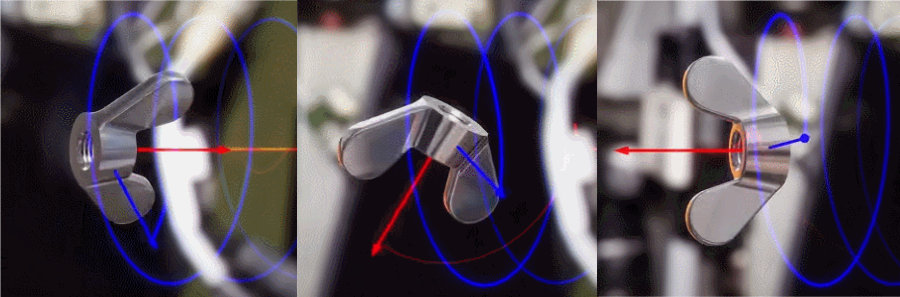
\includegraphics[width=0.9\textwidth]{dzhani.jpg}
\end{center}
   \caption{A depiction of the Dzhanibekov effect \cite{28}.}
\label{fig:10}
\end{figure*}

The principle behind a rapid change in Earth's rotational axis lies in the physics of rotating objects. The canonical example of this is the Dzhanibekov effect, discovered by Russian astronaut Vladimir Dzhanibekov \cite{37}, and depicted in Figure \ref{fig:10}. An object that is not spinning perfectly on one of its three principal axes of inertia will not maintain a fixed rotational axis. If it is rotating close to its second principal axis, it will undergo what appear to be sudden shifts in rotation. While this is not exactly what we believe happens during Earth's rapid flips, the point is that in the absence of external forces, only rotational physics can explain a rapid change in rotational axis of the Earth.

To be precise, the Earth almost certainly does not experience a simple and uniform Dzhanibekov effect. If this were the case, we would be able to detect a gradual shift in Earth's rotational axis over time. Rather, we believe that the Earth experiences periodical, sudden disruptions in its physical structure, leading to a decoupling of its "outer rotational" (crust/mantle) and "inner rotational bodies" (core). Without an external input, the law of conservation of angular momentum states that Earth cannot suddenly change its rotational axis, so a decoupling of outer and inner rotational bodies is one of the few things, barring an external impact on Earth, that could cause a sudden and abrupt flip.

The specific process which drives the internal disruption in the Earth is believed to be a state change in the structure of iron that makes up the core of the Earth (Figure \ref{fig:11}). The inner core is made up of hexagonal close-packed Iron (Fe) \cite{141}. As this hcp-Fe is converted into a liquid metallic state, it releases kinetic energy, and is sloughed into the outer core. This phase change reduces the core's magnetic permeability, weakening the geomagnetic field, and releases heat, creating LLVP (large low-velocity shear province) structures (Figure \ref{fig:12}) \cite{38} in the mantle, and heating up the Earth's surface via the abyssal oceans. Both trends have been well documented in recent centuries and are discussed later in this paper.

\begin{figure*}[t]
\begin{center}
% \fbox{\rule{0pt}{2in} \rule{.9\linewidth}{0pt}}
\includegraphics[width=1\textwidth]{layers.jpg}
\end{center}
   \caption{Depiction of the inner Earth processes that lead to the ECDO flip \cite{129}.}
\label{fig:11}
\end{figure*}


\begin{figure}[t]
\begin{center}
% \fbox{\rule{0pt}{2in} \rule{0.9\linewidth}{0pt}}
   \includegraphics[width=1\linewidth]{llvp.jpg}
\end{center}
   \caption{A detailed visual of the LLVP under South Africa \cite{28}.}
\label{fig:12}
\label{fig:onecol}
\end{figure}


This same process inside the Earth, occurring in a reverse fashion, is also believed to drive the shift back to Earth's current rotational state relatively soon after the flip occurs.

\section{Evidence for an Impending Earth Flip}

There is strong reason to believe that we are on the brink of another Earth flip. A cataclysm has not occurred for several millennia, which is approximately the frequency with which these events seem to happen based on historical accounts and data. The strongest data supporting an impending flip comes from recent geomagnetic data, which indicates that the Earth's geomagnetic field has been weakening for approximately two thousand years. This weakening has been accelerating and has reached alarming rates in the last few decades.

Depicted in Figure \ref{fig:14} is the geomagnetic field of Earth in 1590 and 2025 \cite{125,126}. As shown in the figure, the field has weakened significantly.

Another metric for the weakening geomagnetic field is the position of the geomagnetic north pole (Figure \ref{fig:13}). Geomagnetic north has historically been located in the Canadian Arctic. However, it has been wandering slowly over the last several centuries, and accelerated significantly a few decades ago. It is now moving rapidly towards Russia at a rate of 55 kilometers per year \cite{124}.

\begin{figure*}[t]
\begin{center}
% \fbox{\rule{0pt}{2in} \rule{.9\linewidth}{0pt}}
\includegraphics[width=0.9\textwidth]{saa.jpg}
\end{center}
   \caption{A depiction of the weakening geomagnetic field from 1590 to 2025. Calculated using the gufm1 and IGRF-14 models \cite{125,126}.}
\label{fig:14}
\end{figure*}

\begin{figure}[t]
\begin{center}
% \fbox{\rule{0pt}{2in} \rule{1\linewidth}{0pt}}
   \includegraphics[width=1\linewidth]{npw.jpg}
\end{center}
   \caption{The position of the geomagnetic north pole from 1590 to 2025, depicted in 5-year increments \cite{142}.}
\label{fig:13}
\label{fig:onecol}
\end{figure}

\begin{figure}[t]
\begin{center}
% \fbox{\rule{0pt}{2in} \rule{1\linewidth}{0pt}}
   \includegraphics[width=1\linewidth]{ocean-highlight.jpg}
\end{center}
   \caption{Deep ($>$2000 m depth) ocean warming rates from 1991 to 2010, circled in red \cite{132}.}
\label{fig:15}
\label{fig:onecol}
\end{figure}

Earth's magnetic field is believed to be generated by an inner dynamo - circular columns of magma currents moving in the Earth's outer core due to its rotation \cite{123}. A weakening geomagnetic field is a symptom of disruptions deep inside the Earth. According to the ECDO theory, these disruptions expel heat and eventually lead to the decoupling of the mantle and the core, causing an Earth flip \cite{1}.

There is considerable data corroborating the presence of exothermic inner Earth processes. A warming Earth is documented in rising continental and oceanic surface temperatures \cite{127,128}, rising atmospheric CO2 levels moving in sync with Earth's heat plumes \cite{129,130}, and a decrease in global sea ice extent \cite{131}. The data suggests that rising CO2 levels and temperatures are not the cause of "man-made" climate change but rather, downstream effects of an exothermic core \cite{129}.

Most significantly, studies of warming rates in the deep ocean (depth $>$2000 meters) show that not only are the deep oceans warming, the strongest warming rates are found in the abyssal layer (4000 - 6000 m). This deepsea warming has a centroid below 4000 meters \cite{132,129}, which would not be possible if the oceans were being heated from above by the atmosphere. Such data provides strong support to the case that recent climate and geomagnetic changes are driven by processes deep inside the Earth. Figure \ref{fig:15} depicts global deep-ocean warming rates from 1991 to 2010 \cite{132}.

\section{Modeling The Impending Earth Flip}

\begin{figure}[b]
\begin{center}
% \fbox{\rule{0pt}{2in} \rule{1\linewidth}{0pt}}
   \includegraphics[width=1\linewidth]{saa-crop.jpeg}
\end{center}
   \caption{A tipping point calculation based on the South Atlantic Anomaly points to a date of March 13, 2059 \cite{125,126}.}
\label{fig:16}
\label{fig:onecol}
\end{figure}

Predicting the timing of Earth's next flip is a complex task. Currently, the best model we have for this lies in the geomagnetic field of the Earth - the South Atlantic Anomaly (SAA). This region over the South Atlantic has the weakest geomagnetic field strength and is defined as the area with a field strength below 32,000 nanoteslas \cite{135}, which was the weakest field value in 1590. The South Atlantic Anomaly's surface area increased from 1\% of Earth's surface in 1590 to 21\% in 2025 \cite{136}.

In order to get an estimate for when the Earth could flip, I fit the SAA surface extent data to a power-law tipping point equation, which models a complex system approaching a critical transition, at which the system undergoes a dramatic and abrupt change. My calculations yielded a predicted tipping point date of March 13, 2059 (Figure \ref{fig:16}). This prediction would become more and more accurate the closer we get to the transition \cite{136}.

Other metrics such as rotational axis wander, weather anomalies, and seismic and volcanic data can also help us get a better prediction of when the next Earth flip may happen.

\section{ECDO Historical Timeline}

While establishing an exact timeline for past ECDO events is difficult, it seems that there were at least 2 ECDO events during the Holocene. Note the account told by Herodotus from Egyptian priests that, \textit{"from the first king down to this priest of Hephaistos who reigned last, there had been three hundred and forty-one generations of men... In this time they said that the sun had moved four times from his accustomed place of rising, and where he now sets he had thence twice had his rising, and in the place from whence he now rises he had twice had his setting"} \cite{32}. Plato, who lived during the fifth century BCE \cite{111}, stated that after the flood that drowned Atlantis in a single day and night 9,000 years before, \textit{"there have since been many deluges, and the remnant who survived in the mountains were ignorant of the art of writing, and during many generations were wholly devoted to acquiring the means of life"} \cite{112}, which suggests there were more than two flips since the end of the Younger Dryas circa 9700 BCE. The physical evidence covered throughout this paper and in my research \cite{2} provides ample evidence for Plato's account.

The most recent candidate date for an ECDO flip is during the period of 2300 to 1600 BCE, to which many cataclysmic flood accounts (Gun-Yu \cite{113,114,115}, Ogyges \cite{116,117}, Peru \cite{118,119}, Exodus \cite{120}), civilizational destructions and abandonments (Mohenjo-Daro \cite{121}, Minoan Crete\cite{100,101}) and physical anomalies (bond events \cite{122}, 4.2 kiloyear event \cite{90}) have been dated. There is no ample convergence of evidence more recent than this suggesting a major catastrophic event.

\section{Conclusion}

Operation NANOOK was a Cold War reconnaissance effort of the United States to map the Arctic and the northern Soviet Coast after WWII \cite{137}. During their investigation, they discovered that the magnetic pole was 125 to 200 miles north of where it was supposed to be based on findings from earlier expeditions. Accordingly, \textit{"Among the government scientists, the question arose as to what would happen when the magnetic and geographic poles coincided. To answer this, under the project control of Dr. Paul A. Siple, the Rand Corporation was contracted to conduct lab studies using models of the earth constructed of concentric spheres – an inner sphere representing the electromagnetically-charged molten iron core of the earth whose axis defined the “magnetic” poles; and an outer sphere representing the crust of the earth which rotated around a “geographic” polar axis. It was determined through repeated experimentation that as the “magnetic” pole approached the “geographic” pole, the “magnetic” pole would at some point accelerate its rate of convergence as though pulled toward the “geographic” pole by centripetal force and jump to coincide; but instead of the poles coinciding, the “magnetic” pole would rapidly “flip” around the “geographic” pole, then spin off towards the equator as though by centrifugal force, ending up at a position where the two axes assumed an approximate 89-degree divergence. After this polar “flip” occurred, the axes would then gradually begin to reconverge over a long period of time"} \cite{138,139}.

Subsequently, \textit{"At one of the scientific meetings that Major White attended in the Pentagon in early 1948, the scientists discussed the advisability of alerting the public to the pending polar-flip phenomenon. None of the scientists would agree to withhold the information from the public; but, on the other hand, neither could they agree on how to release it. The knowledge of this phenomenon, some felt, could in itself destroy the moral fiber of society. Their fears were apparently unfounded when, in the early 1950s, information about the flip phenomenon was released in both a newspaper column and a magazine article, but surprisingly generated no responses from an apparently stunned, parochial or incredulous public"} \cite{138,139}.

Why are we not paying attention to this? There is ample reason to believe that the Earth has flipped before. This paper, along with part two of the paper, provide a dense summary of a great convergence of evidence from many areas suggesting that this is the case, such as flood stories all over the world, salt and marine fossils covering the continents, ancient underground shelters, animal remains, and cataclysmic geological landscapes. Humans are supposedly hundreds of thousands of years old, yet modern history only goes back several thousand years. Might it not be the case that every so often, the Earth flips, the continents are wiped clean, and we are forced to return to square one - the Stone Age - reducing our records of ancient history to a handful of cataclysmic stories? If so, then preventing this from happening again may be one of humanity's most important tasks.

In closing, I shall leave you with this account recounted in Timaeus, written by Plato, of a conversation between Solon, an Athenian statesman, and Egyptian priests \cite{140}: \textit{"And on one occasion, when [Solon] wished to draw them on to discourse on ancient history, he attempted to tell them the most ancient of our traditions, concerning Phoroneus, who was said to be the first man, and Niobe; and he went on to tell the legend about Deucalion and Pyrrha after the Flood, and how they survived it, and to give the geneology of their descendants; and by recounting the number of years occupied by the events mentioned he tried to calculate the periods of time. Whereupon one of the priests, a prodigiously old man, said, “O Solon, Solon, you Greeks are always children: there is not such a thing as an old Greek.” And on hearing this he asked, “What mean you by this saying?” And the priest replied, “You are young in soul, every one of you. For therein you possess not a single belief that is ancient and derived from old tradition, nor yet one science that is hoary with age. And this is the cause thereof: There have been and there will be many and divers destructions of mankind, of which the greatest are by fire and water, and lesser ones by countless other means. For in truth the story that is told in your country as well as ours, how once upon a time Phaethon, son of Helios, yoked his father's chariot, and, because he was unable to drive it along the course taken by his father, burnt up all that was upon the earth and himself perished by a thunderbolt — that story, as it is told, has the fashion of a legend, but the truth of it lies in the occurrence of a shifting of the bodies in the heavens which move round the earth, and a destruction of the things on the earth by fierce fire, which recurs at long intervals. At such times all they that dwell on the mountains and in high and dry places suffer destruction more than those who dwell near to rivers or the sea; and in our case the Nile, our Saviour in other ways, saves us also at such times from this calamity by rising high. And when, on the other hand, the Gods purge the earth with a flood of waters, all the herdsmen and shepherds that are in the mountains are saved, but those in the cities of your land are swept into the sea by the streams; whereas In our country neither then nor at any other time does the water pour down over our fields from above, on the contrary it all tends naturally to well up from below. Hence it is, for these reasons, that what is here preserved is reckoned to be most ancient; the truth being that in every place where there is no excessive heat or cold to prevent it there always exists some human stock, now more, now less in number. And if any event has occurred that is noble or great or in any way conspicuous, whether it be in your country or in ours or in some other place of which we know by report, all such events are recorded from of old and preserved here in our temples; whereas your people and the others are but newly equipped, every time, with letters and all such arts as civilized States require and when, after the usual interval of years, like a plague, the flood from heaven comes sweeping down afresh upon your people, it leaves none of you but the unlettered and uncultured, so that you become young as ever, with no knowledge of all that happened in old times in this land or in your own. Certainly the genealogies which you related just now, Solon, concerning the people of your country, are little better than children's tales; for, in the first place, you remember but one deluge, though many had occurred previously; and next, you are ignorant of the fact that the noblest and most perfect race amongst men were born in the land where you now dwell, and from them both you yourself are sprung and the whole of your existing city, out of some little seed that chanced to be left over; but this has escaped your notice because for many generations the survivors died with no power to express themselves in writing. For verily at one time, Solon, before the greatest destruction by water, what is now the Athenian State was the bravest in war and supremely well organized also in all other respects. It is said that it possessed the most splendid works of art and the noblest polity of any nation under heaven of which we have heard tell”}.

These same priests, of course, also told Solon about the ancient civilization of Atlantis: \textit{"For all that we have here, lying within the mouth of which we speak, is evidently a haven having a narrow entrance; but that yonder is a real ocean, and the land surrounding it may most rightly be called, in the fullest and truest sense, a continent. Now in this island of Atlantis there existed a confederation of kings, of great and marvellous power, which held sway over all the island, and over many other islands also and parts of the continent; and, moreover, of the lands here within the Straits they ruled over Libya as far as Egypt, and over Europe as far as Tyrrhenia. So this host, being all gathered together, made an attempt one time to enslave by one single onslaught both your country and ours and the whole of the territory within the Straits. And then it was, Solon, that the manhood of your State showed itself conspicuous for valor and might in the sight of all the world. For it stood pre-eminent above all in gallantry and all warlike arts, and acting partly as leader of the Greeks, and partly standing alone by itself when deserted by all others, after encountering the deadliest perils, it defeated the invaders and reared a trophy; whereby it saved from slavery such as were not as yet enslaved, and all the rest of us who dwell within the bounds of Heracles it ungrudgingly set free. But at a later time there occurred portentous earthquakes and floods, and one grievous day and night befell them, when the whole body of your warriors was swallowed up by the earth, and the island of Atlantis in like manner was swallowed up by the sea and vanished"}.

\section{Acknowledgments}

Thanks to Ethical Skeptic, the original author of the ECDO thesis, for completing his insightful, groundbreaking thesis and sharing it with the world. His tri-part thesis \cite{1} remains the seminal work for Exothermic Core-Mantle Decoupling Dzhanibekov Oscillation (ECDO) theory, and contains much more information on the topic than I have covered briefly here.

Thanks to Ankit, who processed the cataclysm compilation data in Table 1.

And of course, thanks to the giants whose shoulders we stand on; those who have done all the research and investigation that made this work possible and worked to bring light to humanity.

\clearpage
\twocolumn

\section{Additional Images}


\begin{figure}[H]
\begin{center}
% \fbox{\rule{0pt}{2in} \rule{1\linewidth}{0pt}}
   \includegraphics[width=1\linewidth]{wave.jpg}
\end{center}
   \caption{A close look at the undercut, parabolic wave erosion on the Khafre pyramid \cite{27}.}
\label{fig:19}
\label{fig:onecol}
\end{figure}

\begin{figure}[H]
\begin{center}
% \fbox{\rule{0pt}{2in} \rule{1\linewidth}{0pt}}
   \includegraphics[width=1\linewidth]{star-stone.jpg}
\end{center}
   \caption{The star map carved into stone in one of the Khufu pyramid shafts \cite{28}.}
\label{fig:20}
\label{fig:onecol}
\end{figure}

\begin{figure*}[t]
\begin{center}
% \fbox{\rule{0pt}{2in} \rule{.9\linewidth}{0pt}}
\includegraphics[width=1\textwidth]{deepsea.jpg}
\end{center}
   \caption{A visual of the deep and abyssal ocean heating anomaly compared to a normal atmospheric ocean heating curve. The overall heating anomaly has been taken from NOAA \cite{147}, the deep and abyssal heating distributions from a Desbruyeres study \cite{132}, and the data processing and visualization by Ethical Skeptic \cite{129}.}
\label{fig:21}
\end{figure*}

\begin{figure*}[t]
\begin{center}
% \fbox{\rule{0pt}{2in} \rule{.9\linewidth}{0pt}}
\includegraphics[width=1\textwidth]{sealevel.jpeg}
\end{center}
   \caption{Sea level shows a 20\% increase in variance over 75 years across 63 stations, indicating an increase in current speed. Surges in sea level variance are concurrent with ocean heat pulses, indicating these may both be caused by heating from deep below the Earth's oceans \cite{2,129}.}
\label{fig:22}
\end{figure*}

\begin{figure*}[t]
\begin{center}
% \fbox{\rule{0pt}{2in} \rule{.9\linewidth}{0pt}}
\includegraphics[width=1\textwidth]{co2.jpg}
\end{center}
   \caption{Atmospheric CO2 ppm has risen consistently over the last 45 years, likely caused by a rise in ocean temperatures. Source: NOAA \cite{148,129}.}
\label{fig:23}
\end{figure*}

\begin{figure*}[t]
\begin{center}
% \fbox{\rule{0pt}{2in} \rule{.9\linewidth}{0pt}}
\includegraphics[width=1\textwidth]{ice.jpg}
\end{center}
   \caption{Global sea ice extent has been shrinking over the last 45 years, due to a warming Earth. Source: ADS \cite{149}.}
\label{fig:24}
\end{figure*}

\clearpage
\twocolumn

{\small
\renewcommand{\refname}{References}
\bibliographystyle{ieee}
\bibliography{egbib}
}

\end{document}
